\section{Background}

\subsection{Overview}
This project is about implementing an E2EE chat system using Signal Protocol. So understanding how Signal Protocol works is essential in both development and reading. Only after having a deep understanding of Signal Protocol, the whole work can be processed smoothly.

This project uses the libsignal-protocol-java package to develop the Signal Protocol part. However, the documentation of it is not enough to support the new developer to use it. Reading related papers, user guide of related commercial products and the source code of the lib is quite useful.

In this chapter, the report will have a introduction about how Signal Protocol works and how it's implemented in related existing commercial products.

In section 3.2.1, the report presents the Double Ratchet algorithm and gives an introduction of how it works. Section 3.2.2 presents how X3DH algorithm works in Signal Protocol. This two algorithms constitute the core of the Signal Protocol. Finally, section 3.2.3 shows how the whole Signal Protocol works by using this two algorithm.

\subsection{Signal Protocol}
The Signal Protocol is designed by Moxie Marlinspike and Trevor Perrin from Open Whisper Systems\footnote{https://whispersystems.org/}. Open Whisper Systems wanted to develop a new end-to-end encryption standard which works in both synchronous and asynchronous messaging environments \citep{SignalRef1}. The goals of Signal include end-to-end encryption and advanced security properties such as forward secrecy and future secrecy \citep{SignalRef2}.

The core parts of Signal Protocol can be divided into Double Ratchet algorithm \citep{DR} and X3DH algorithm \citep{X3DH}. This two guarantee the essential features of Signal Protocol such as forward security, future security and asynchronous.

\subsubsection{Double Ratchet}
The Signal Protocol is designed to solve one of problems that once the hacker cracks one of the encrypted packages, all of the packages before or after will be leaked. The best solution is changing the cipher key in each transmission round. Each cipher key is used once to encrypt or decrypt the messages. So the how to ensure that the generated key cannot be used to refer the previous and subsequent ones is important.

KDF chain \citep{DR} is a core concept in the Double Ratchet algorithm, which is used as a ratchet. It takes a secret, random KDF key and some input data and then returns one key used as a new KDF key for the next chain as well as an another output key. As the ratchet's name shown, the output data is always indistinguishable from random if the input key is not known which provides the resilience: the adversary cannot refer the output key without the input key. Also, the KDF chain has the forward security, although the adversary obtains a KDF key, it's hard to refer to the previous one. 

Until now, the KDF chain which can be called ratchet also provides one-direction security: forward security. The break-in recovery feature of it is the basic of future security it provides: although the adversary obtains a KDF key, it appears random as long as the future inputs have sufficient entropy.

One KDF chain is one ratchet, so Double Ratchet is formed by two KDF chain. One is used as a root chain which is also called DH Ratchet, the other one is used as a sending or receiving chain which is also called Symmetric Ratchet. This two ratchets constitute Double Ratchet algorithm which provides the forward security and future security \citep{DR}.

\subsubsection{X3DH}
The Signal Protocol is designed to work in both synchronous and asynchronous messaging environments. It looks like two parties using Double Ratchet to get the same messaging cipher key needs to be both online in the meanwhile. The key of two parties maintain the same ratchet states is having the same initialize chain key in each KDF chain.

Once the two parties calculating the same chain key at the beginning, they can maintain the same ratchet states. The sender's sending chain corresponds to the receiver's receiving chain. Sender does a ratchet step in sending chain after sending each message while the receiver does a same ratchet step in receiving chain after receiving each message. That guarantees the Double Ratchet can work properly in both two parties.

So the essential thing is using a key agreement protocol \citep{X3DH} to calculate the same first chain key in asynchronous environment. X3DH is developed to solve it. It's also called Extended Triple Diffie-Hellman Algorithm. This protocol requests user to generate several keys called key bundle for further calculation. Each party generates a long-term identity key, a mid-term signed pre key and several one-time pre keys. The public keys used within an X3DH protocol run must either all be in X25519\footnote{https://tools.ietf.org/html/rfc7748} form or X448\footnote{https://tools.ietf.org/html/rfc7748} form.
Then user needs to send this key bundle to server for further pairwise chat initialization.

Assume a situation, Alice wants to send her first message to Bob while Bob is offline currently. First Alice requests Bob's key bundle from the server, Alice also needs to load her own key bundle and generate a pair of ephemeral key \citep{X3DH} in the meanwhile. We define the keys used in this process as following:
\begin{itemize}
\item IKa: Alice's private identity key
\item EKa: Alice's private ephemeral key
\item IKb: Bob's public identity key
\item SPKb: Bob's public signed pre key
\item OPKb: Bob's public one-time pre key
\end{itemize}
And then Alice will start to calculate as following:
\[ DH1=DH(IKa, SPKb) \]
\[ DH2=DH(EKa, IKb) \]
\[ DH3=DH(EKa, SPKb) \]
\[ (Optional) DH4=DH(EKa, OPKb) \]
\[ SK = KDF(DH1 || DH2 || DH3 || DH4) \]
The SK is the master secret result calculated by X3DH and will be used as the first root key in root chain. To make sure that Bob can calculate the same master secret, Alice will send her initial message to Bob with her key bundle including Alice's public identity key, Alice's public ephemeral key and the identifier stating which of Bob's pre keys Alice used.

Once Bob received the initial message from Alice, he will use Alice's public key bundle to calculate the same master secret and delete the corresponding one-time pre key in his stores. Until now, both parties having the same initial root key for further ratchet steps in asynchronous environment.

\subsubsection{Whole process}
After having an overview with Double Ratchet and X3DH algorithm, it's clear to understand how the whole Signal Protocol works. This section presents the work process of Signal Protocol in different situations via the graphic and text combination.

\begin{enumerate}[label=(\roman*)]
\item Initializing Situation

When sender wants to send the first message to the receiver, Signal Protocol needs to initialize the pairwise chat. On the first step, sender requests receiver's key bundle from server, and then uses X3DH algorithm to calculate the master secret as the initial root key in root chain. The figure 3.1 presents this process in detail.

\begin{center}
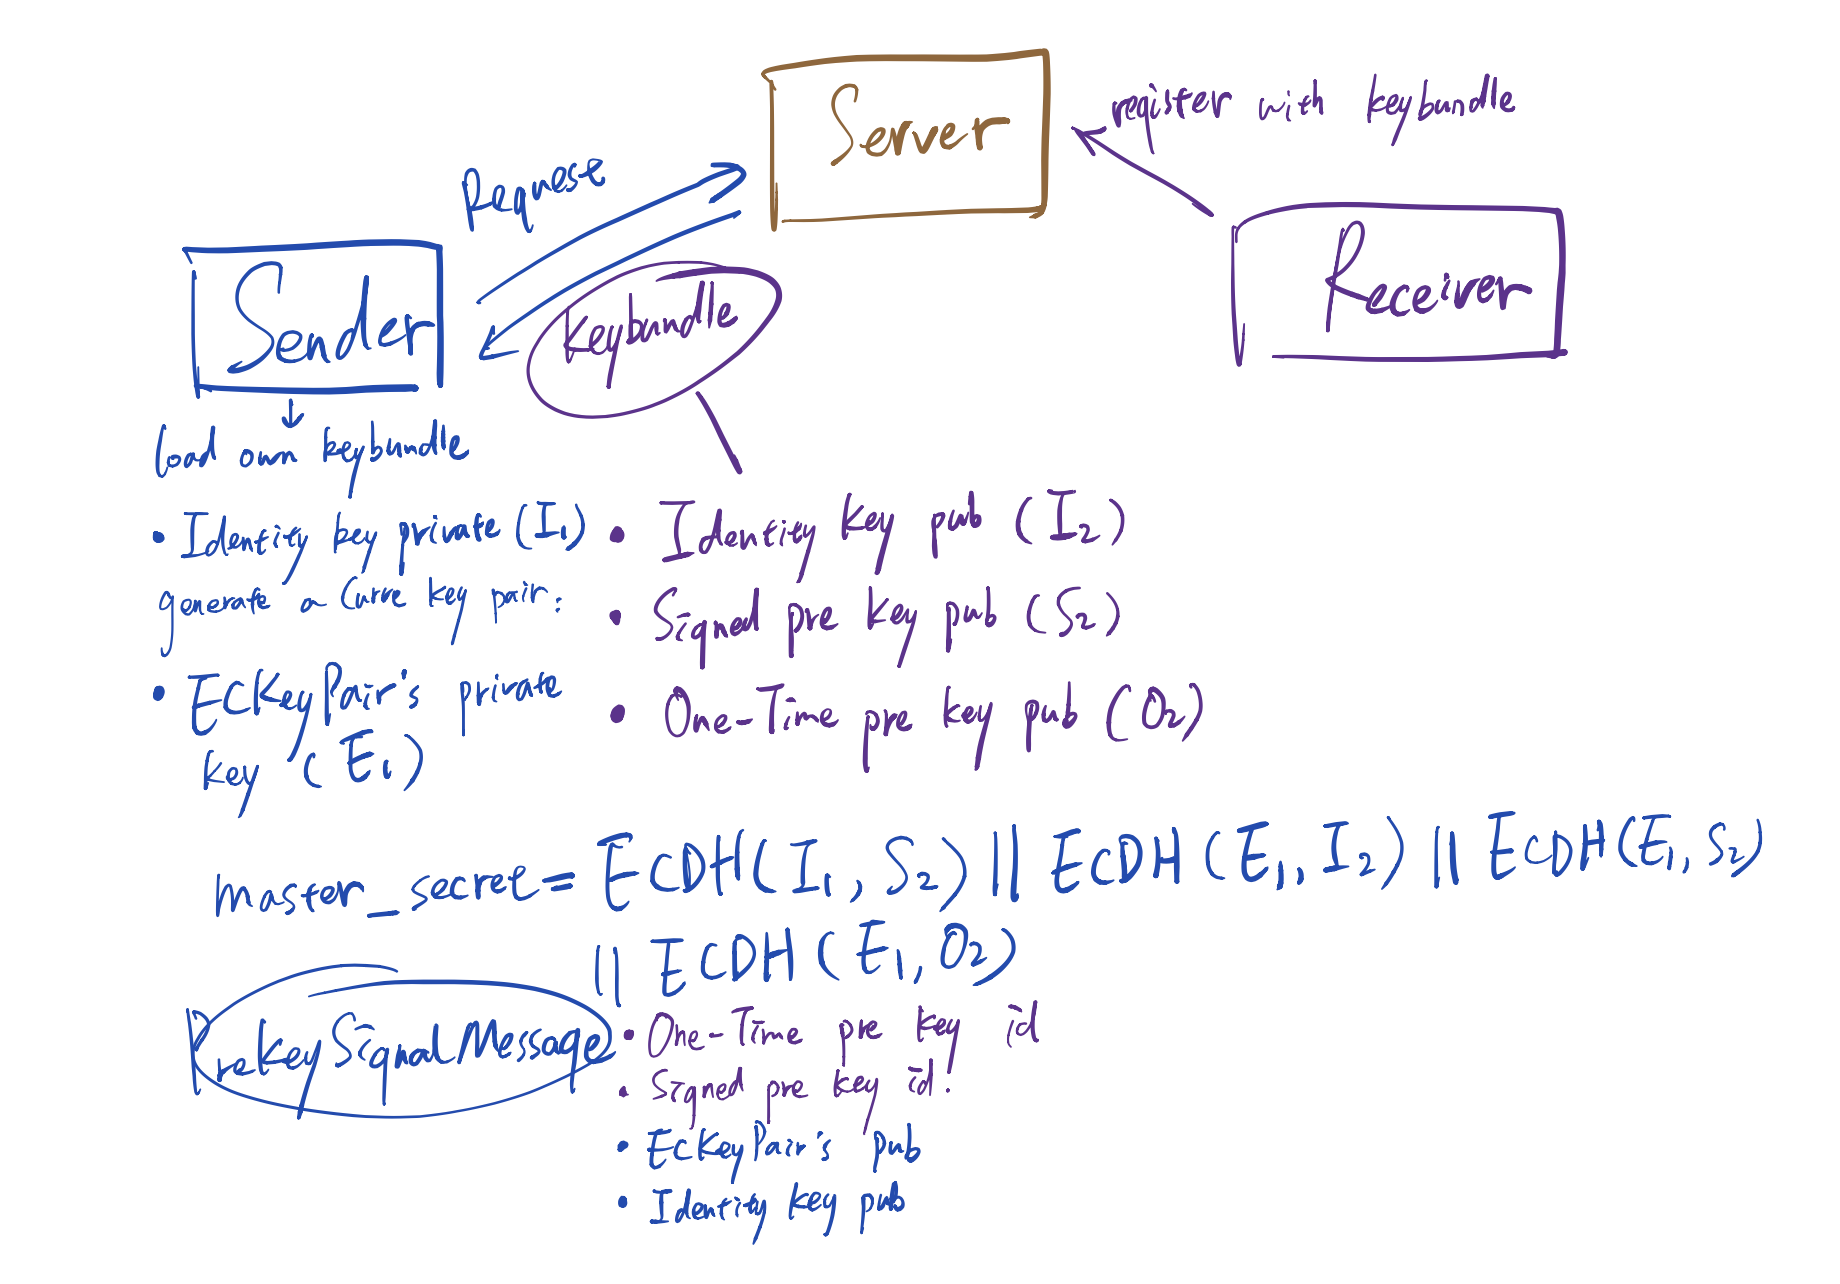
\includegraphics[scale=.5]{../3-Background/resources/X3DH.png}\\
Figure 3.1: \textit{Sender uses Extended Triple Diffie-Hellman Algorithm to initialize the pairwise chat}
\end{center}

Once the master secret is calculated, the sender needs to send his public identity key, the generated public ephemeral key and the receiver's pre keys identifier with the initial message to the receiver.

As mentioned before, the master secret obtained from X3DH is used as the first root key in root chain. Then sender needs to do the first ratchet step in Double Ratchet. The Double Ratchet is formed by DH ratchet and symmetric ratchet. The symmetric ratchet's first chain key is the output of DH ratchet, so sender needs to do the stepping in DH ratchet first. To provide the break-in recovery feature which also means future security, the DH ratchet needs an encrypted input as "salt" in the KDF algorithm. The sufficient entropy of input make the output of KDF appears random which can be used safety as the first chain key in sending or receiving chain.

The input of DH ratchet needs to have enough entropy while it also needs the confidentiality and consistency. So asymmetric encryption is a good solution to solve it. In every messaging package's header, there is a public rathcet key which is used by users to calculate the secret output via DH algorithm. In the initializing situation, receiver's public signed pre key is used as public ratchet key. The sender needs to generate a pair of ratchet keys in the meanwhile and uses the private key of it with the receiver's public signed pre key to do the DH algorithm. The output of it that provides sufficient entropy is used as the input of KDF in DH ratchet's root chain. When sending the message, the sender will send the public key of generated ratchet key pair in message header to make sure the receiver can calculate the same input of KDF in DH ratchet. This process is also called ratcheted key exchange \citep{RatchetedKeyExchange}.

After doing the stepping in DH ratchet, root chain generated a new root chain key and a reliable output. The output is used as the first chain key in the second symmetric ratchet which means the first chain key of sending chain or receiving chain. Because the DH ratchet has already added sufficient entropy, so the output of it which is used as the input of symmetric ratchet is reliable that there is no need to add other entropy in symmetric ratchet. So the inputs of symmetric ratchet can be a constant which are usually 0x01 and 0x02. To get the message cipher key, the symmetric ratchet needs to do another stepping by using the KDF in sending chain. One stepping gets a message key which can be used to encrypt the message and once the encryption is completed, the used message key will be deleted immediately to provide the forward security. If the sender wants to send other messages in the same round, the only thing needs to do is doing the corresponding stepping in sending chain to get the right message keys. The figure 3.2 presents the whole process in detail.

\begin{center}
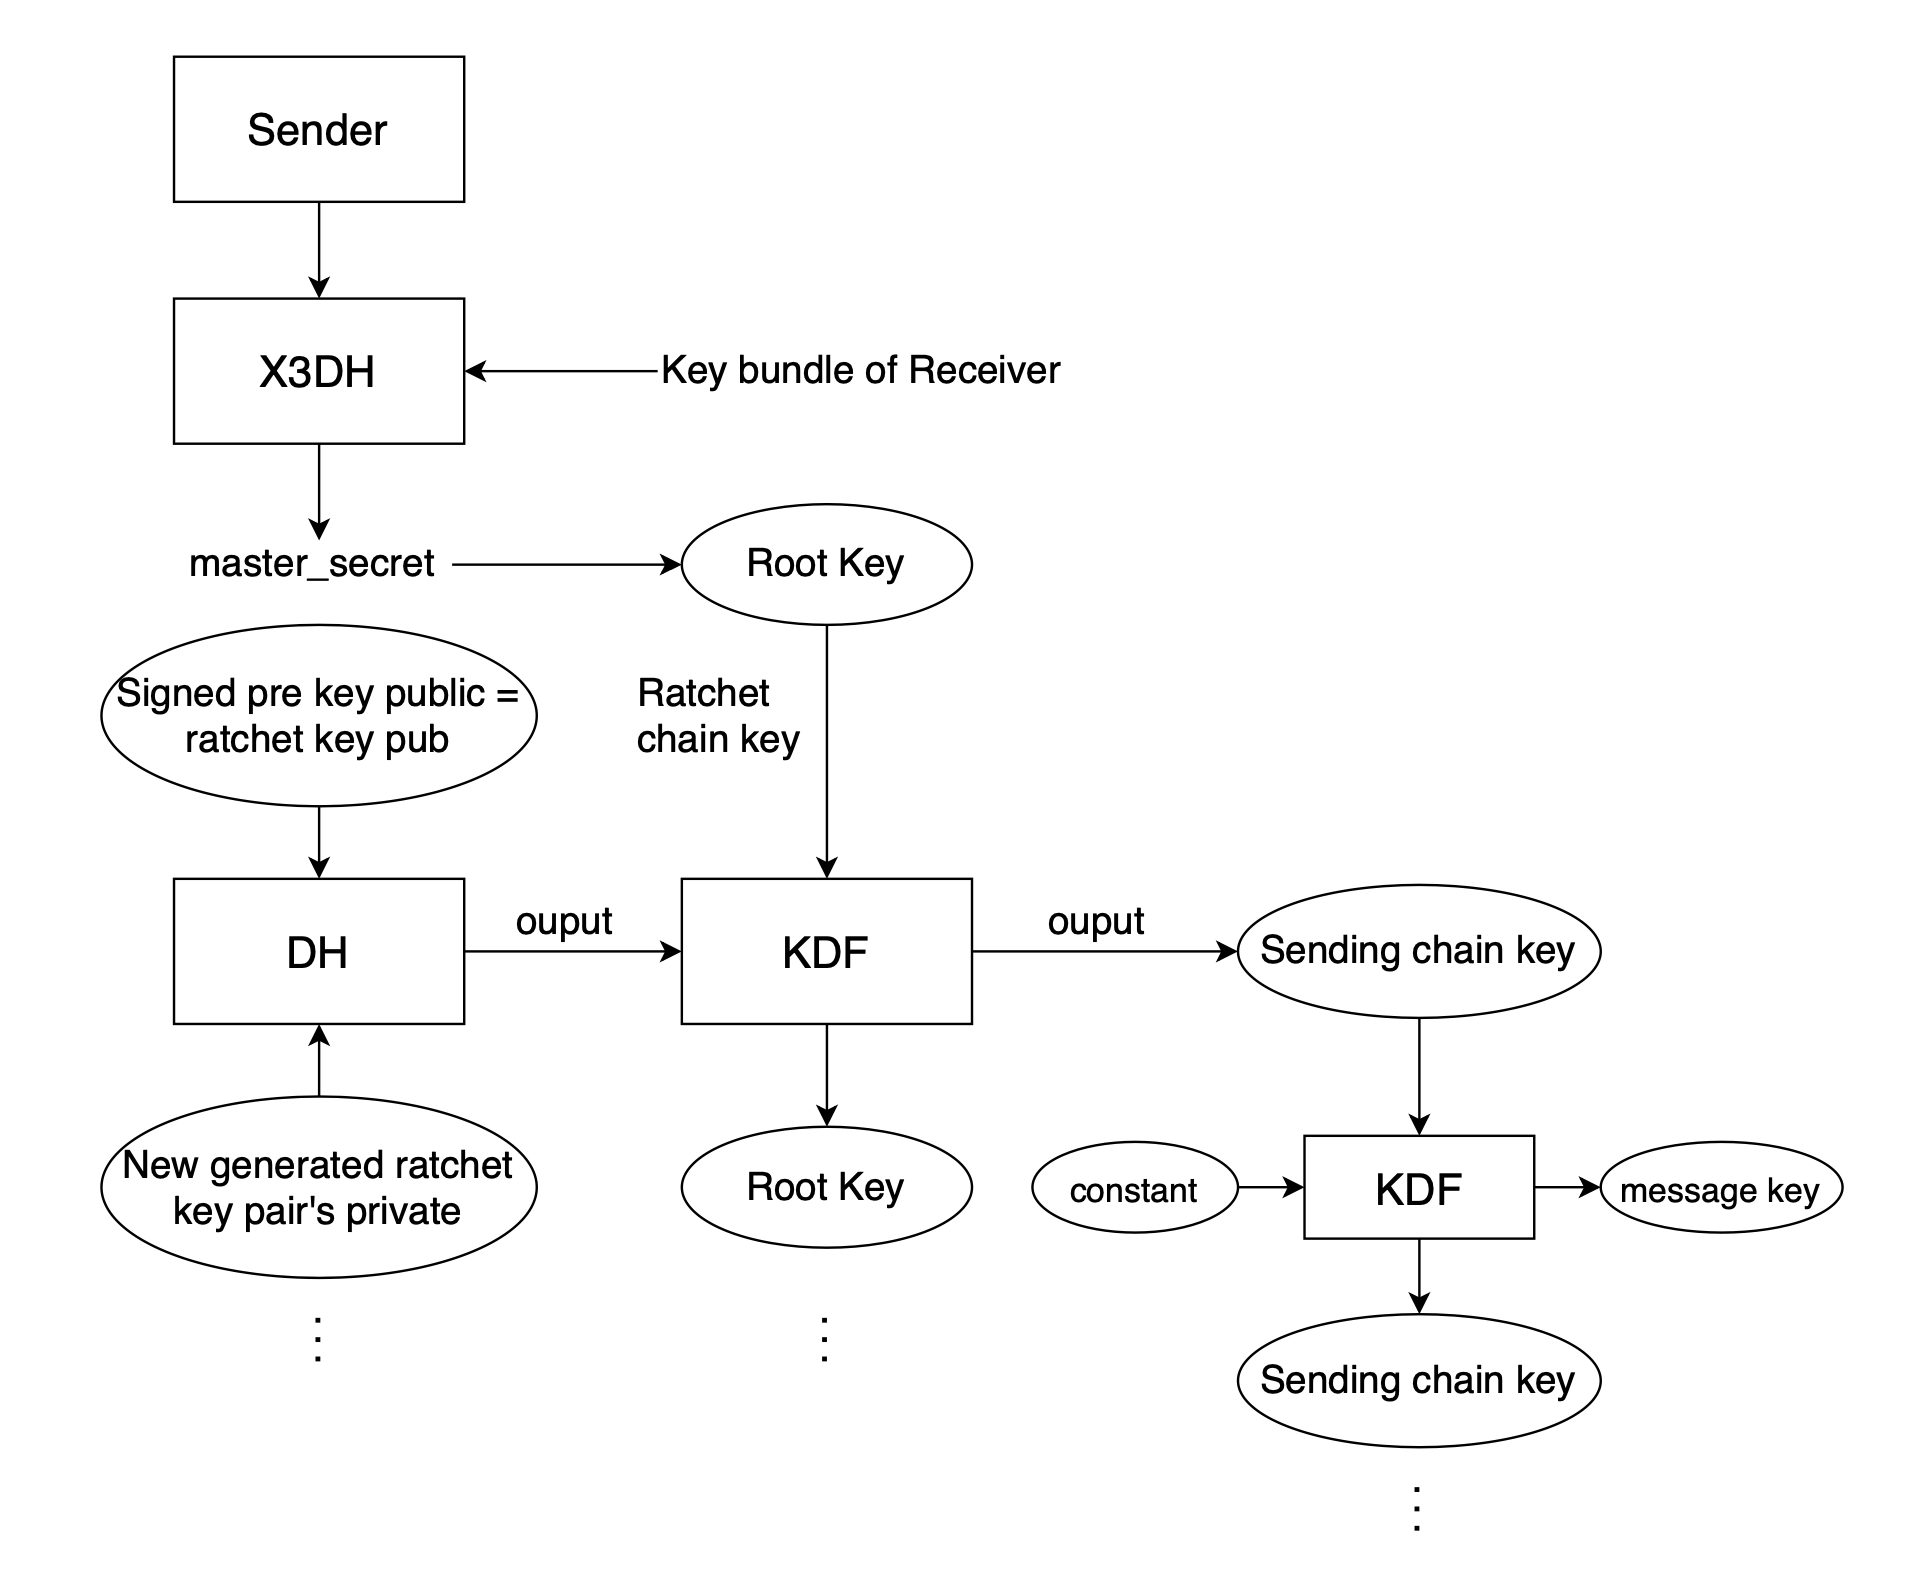
\includegraphics[scale=.5]{../3-Background/resources/DH-init.png}\\
Figure 3.2: \textit{Sender uses the Double Ratchet to encrypt the messages in the initializing situation}
\end{center}

\item Receiving Situation

In the situation that the receiver receives the encrypted messages from sender and wants to decrypt them, if the messages include the X3DH parameters, the receiver needs to calculate the root key first, or the receiver extracts the public ratchet key from message header for further decryption.

Once the public ratchet key is extracted, the receiver needs to judge it with the ratchet states first: if the public ratchet key has the corresponding receiving chain. In the situation that there is not receiving chain corresponds to the received public ratchet key, the receiver uses the old private ratchet key with the received public ratchet key to calculate an output via DH algorithm. Then the receiver uses the output as the input of KDF in DH ratchet's root chain to do a stepping. The output of DH ratchet's KDF will be used as the first chain key in symmetric ratchet's receiving chain as mentioned in initializing situation. Later, the receiver will do the right stepping in receiving chain to obtain the right message key which can be used to decrypt the received messages. Also, for the forward security, once the message key decrypted the messages, it will be deleted immediately. In the other situation that there is a corresponding receiving chain to the received public ratchet key, the receiver gets the right receiving chain and does the proper stepping in symmetric ratchet's receiving chain to get the correct message key.

The Signal Protocol is also designed to handle the out of order messages that may be caused by network delay. If the receiver receives the latter message before the former message, when the symmetric ratchet is doing the corresponding stepping, it will store the generated but never used message key with associated count. Once the former message arrives, the receiver will get the correct message key from stores to decrypt it. The figure 3.3 presents the Double Ratchet's work process in receiving situation.

\begin{center}
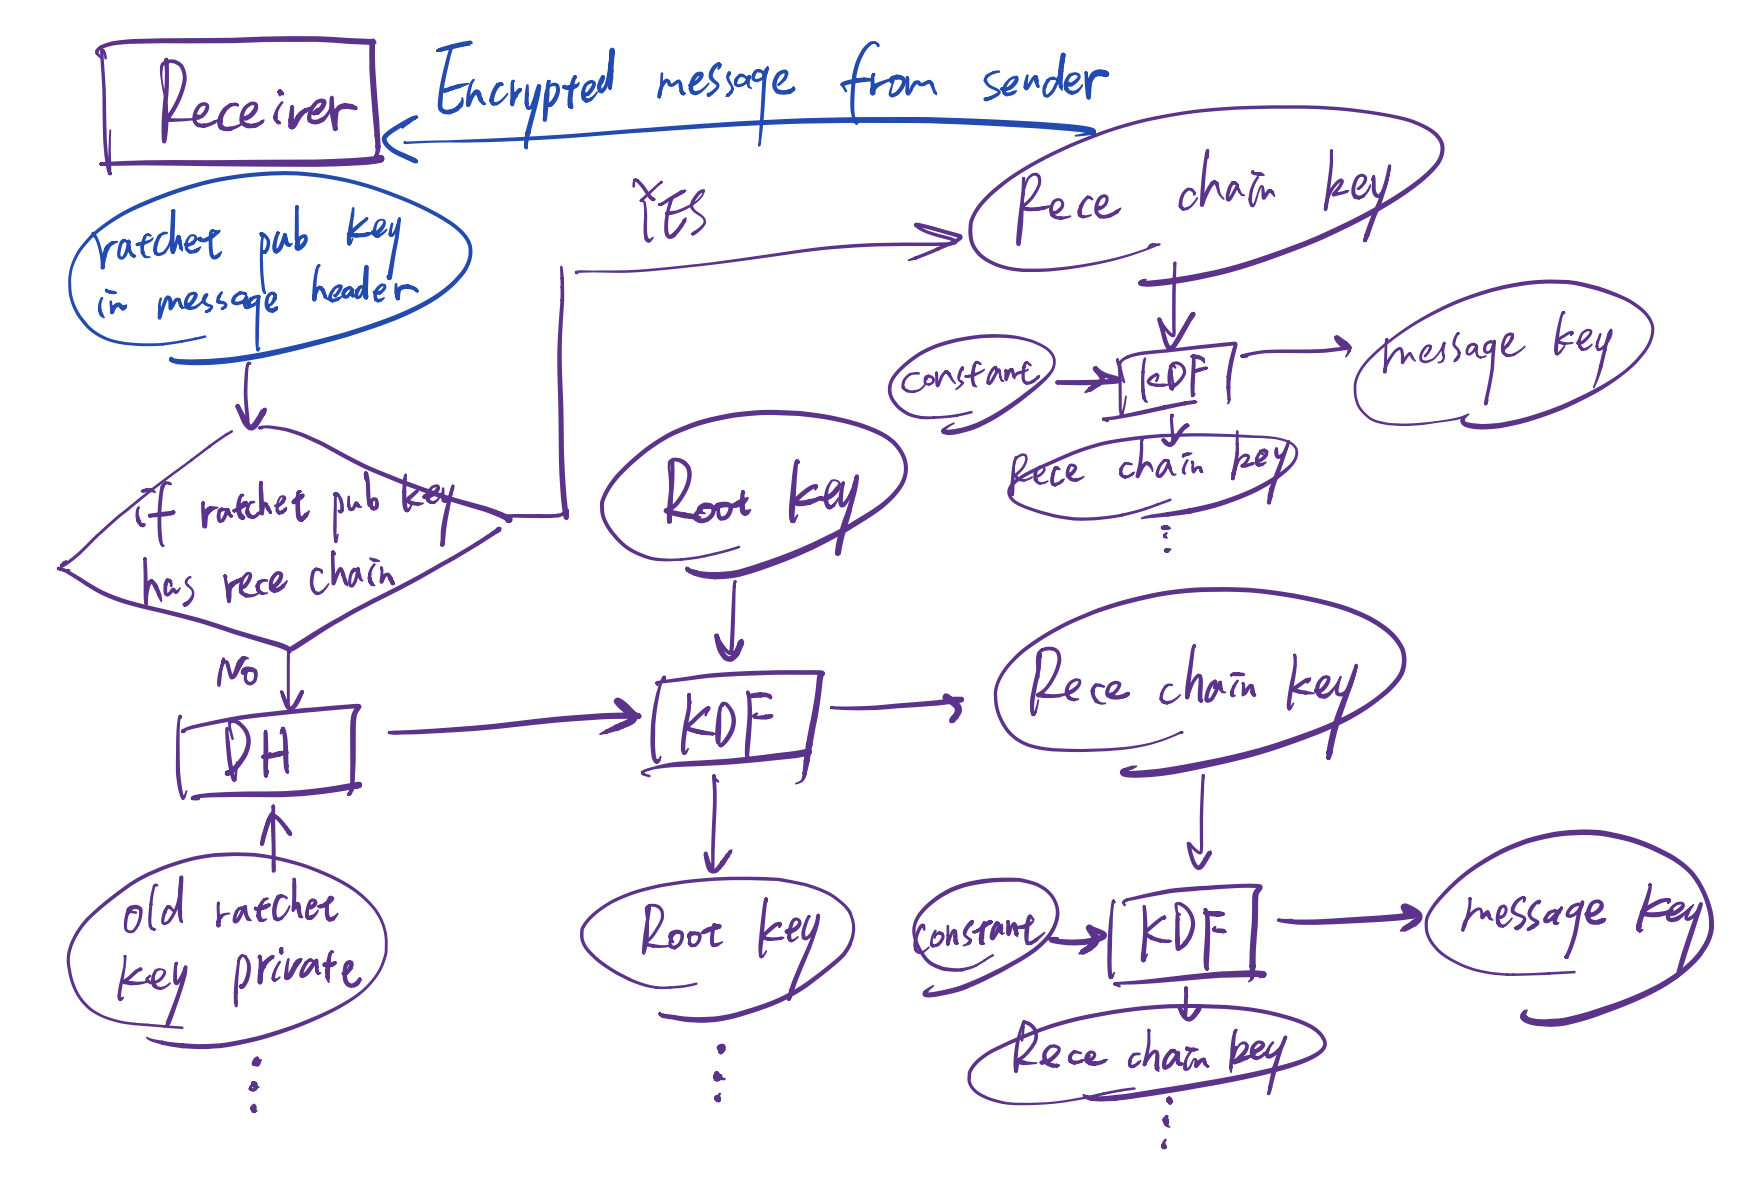
\includegraphics[scale=.5]{../3-Background/resources/DH-rece.png}\\
Figure 3.3: \textit{Receiver uses Double Ratchet to decrypt the messages}
\end{center}

\item Sending Situation

In the situation one party wants to send an encrypted message to others, it's always necessary to generate a new ratchet key pair. The user will extract the public ratchet key in latest message header first, and uses it with the private key of new generated ratchet key pair to calculate the output of DH algorithm. Then the output will be used as the input of the KDF in DH ratchet's root chain and the later steps are almost the same as mentioned in other situations before. Once the message is encrypted and prepared to be sent, the sender needs to add the public key of generated ratchet key pair in message header to make sure the receiver can do the same ratchet stepping. The figure 3.4 presents this process in detail.

\begin{center}
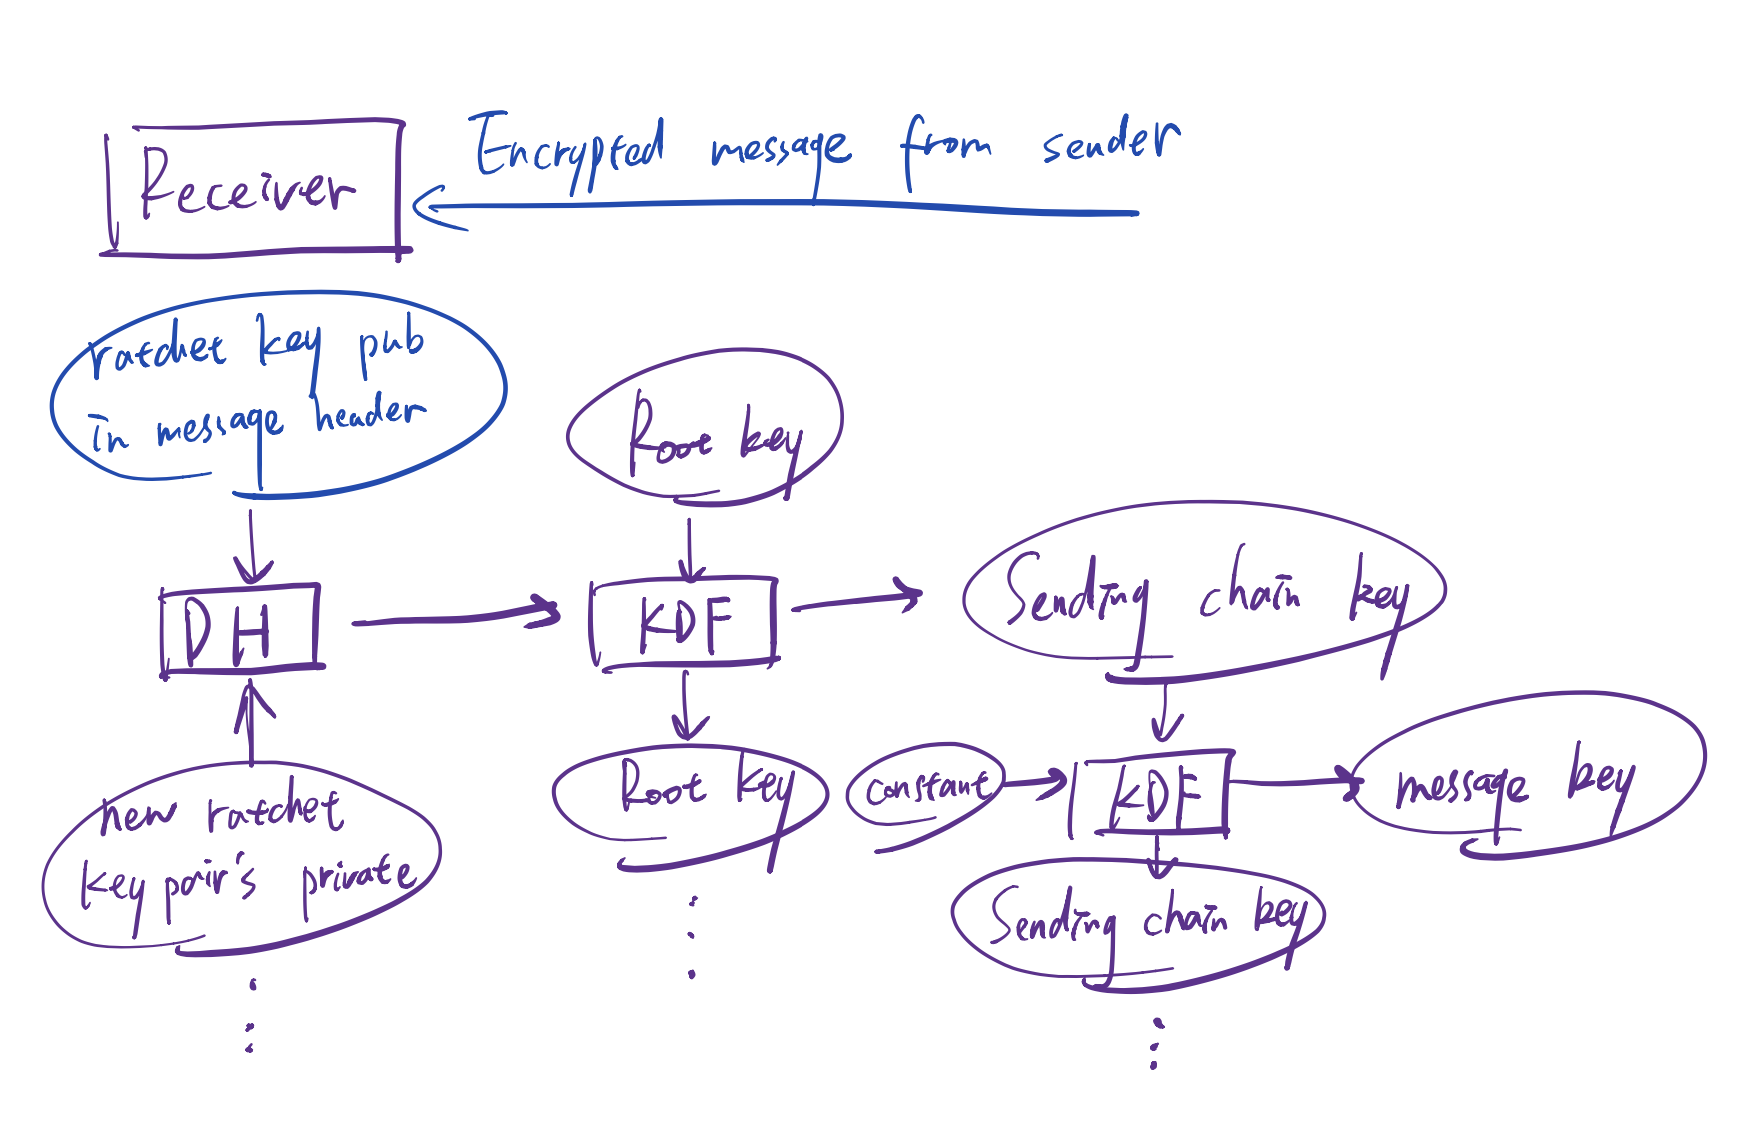
\includegraphics[scale=.5]{../3-Background/resources/DH-send.png}\\
Figure 3.4: \textit{User uses Double Ratchet to send the messages}
\end{center}

\end{enumerate}

\subsection{Related work}
The Signal Protocol is a certain reliable protocol nowadays, there are several applications related to it in our life.

WhatsApp upgrades its application based on Signal Protocol in February 2017 to secure its content. Signal Protocol also has a same name chat application called Signal, which has been used by a lot of people since 2013.

 This project also borrows some strategies from WhatsApp to handle different problems in different situations, like group chat and pairwise chat's fingerprint verification function. However, since this project is developed from an existing chat system, the defect is the communication between the server and the client is special, each side has their own way to handle different type of packages. So the client cannot communicate with other Signal Compatible Server which is a regret. But the idea of Signal Protocol has been implemented in this project, it really improves the security of users' communications.

\clearpage